\documentclass{beamer}

\usepackage{hyperref}

\usetheme{Madrid}
\setbeamertemplate{navigation symbols}{}
%\setbeamercovered{transparent}

\newcommand{\email}[1]{\texttt{#1}}


\title[Using Cloud9]{Using BRIDGES Cloud9 Service}

\author[Erik Saule]{{\bf Erik Saule}\\\email{esaule@uncc.edu}}

\institute[BRIDGES]{BRIDGES Workshop}

\date{}

\begin{document}

\maketitle

\begin{frame}{\url{https://846334404766.signin.aws.amazon.com/console}}
  Use provided credentials.
  
  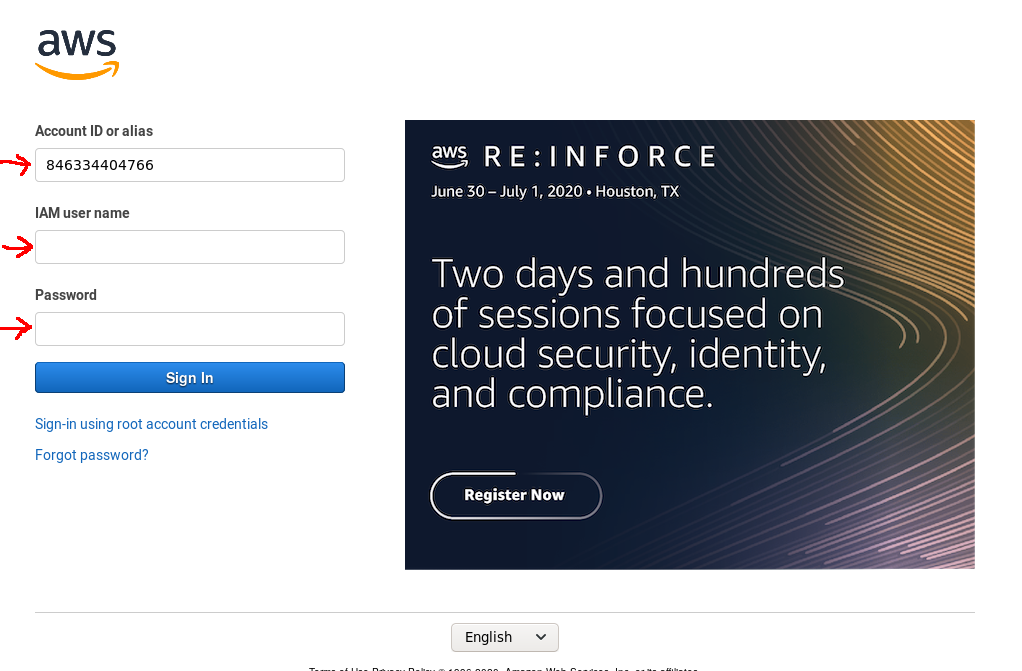
\includegraphics[width=\linewidth]{cloud9_figures/AWSCloud9SignIn.png}

  %account: bridges-user1
  %password: bridges-user
  %up to 50
\end{frame}



\begin{frame}{Make sure you are in US West Orgeon}
  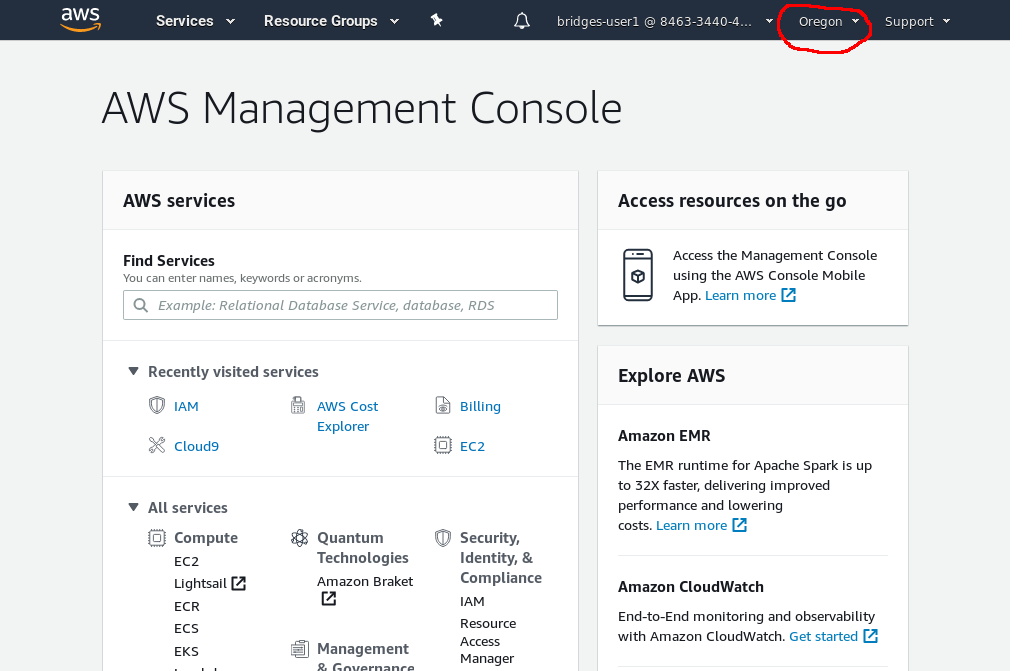
\includegraphics[width=\linewidth]{cloud9_figures/AWSRegion.png}
\end{frame}

\begin{frame}{Select Cloud9}
  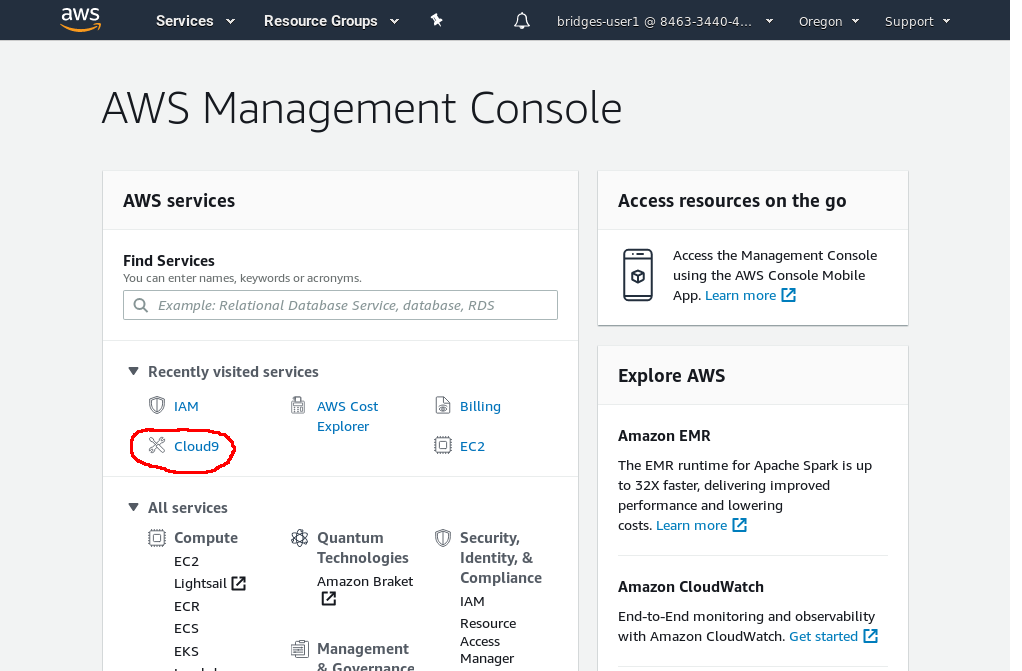
\includegraphics[width=\linewidth]{cloud9_figures/SelectCloud9.png}
\end{frame}

\begin{frame}{Select Open IDE}
  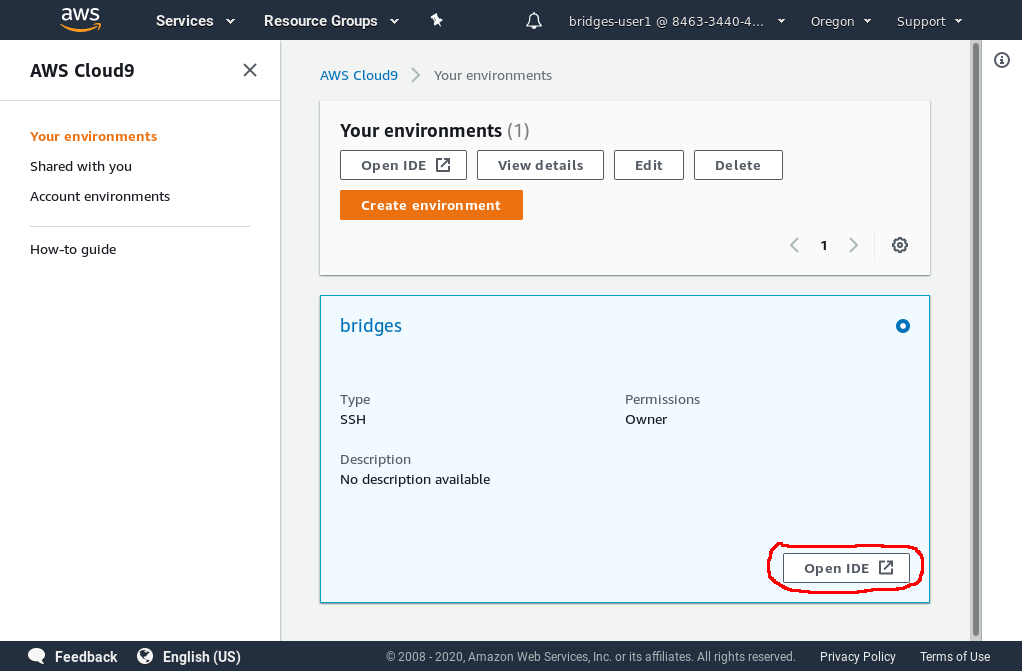
\includegraphics[width=\linewidth]{cloud9_figures/OpenIDE.png}
\end{frame}

\begin{frame}{You Are Ready to JAM}
  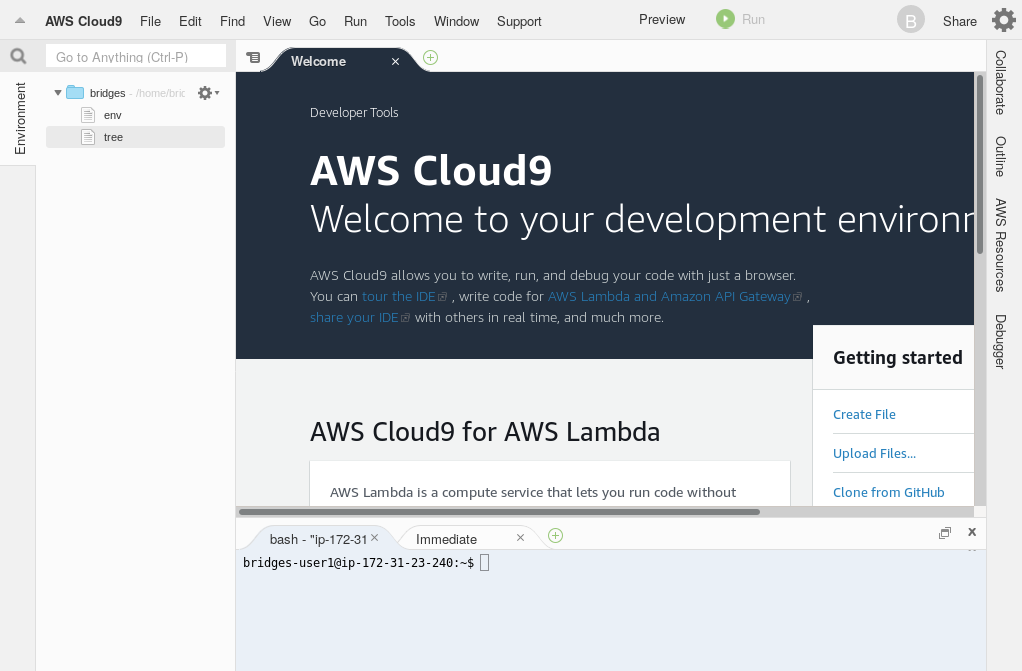
\includegraphics[width=\linewidth]{cloud9_figures/Ready.png}
\end{frame}

\begin{frame}{Compiling/running}
  You should be able to compile and run codes in java and python by clicking on the interface.

  To compile/run c++ codes, open up a terminal (Alt-T), navigate to
  that directory and compile with ``make''.
\end{frame}


\end{document}
